W~celu implementacji przedstawionego algorytmu negocjacji, wykorzystaliśmy język programowania ogólnego przeznaczenia Python w~wersji 3.6 oraz bibliotekę \texttt{SPADE - Smart Python Agent Development Environment}~\cite{spade}. Biblioteka ta upraszcza proces tworzenia agentów oraz obsługuje komunikację między nimi, która oparta jest o~protokół XMPP.

\subsection{Dekompozycja systemu na agenty}
W~przygotowanym systemie możemy wydzielić dwa rodzaje agentów:
\begin{itemize}
    \item agenty zarządcze,
    \item agenty komórek fabryki. 
\end{itemize}

Na rysunku~\ref{fig:agents} przedstawiony został podział na typy agentów w~systemie.

\begin{figure}[h]
    \centering
    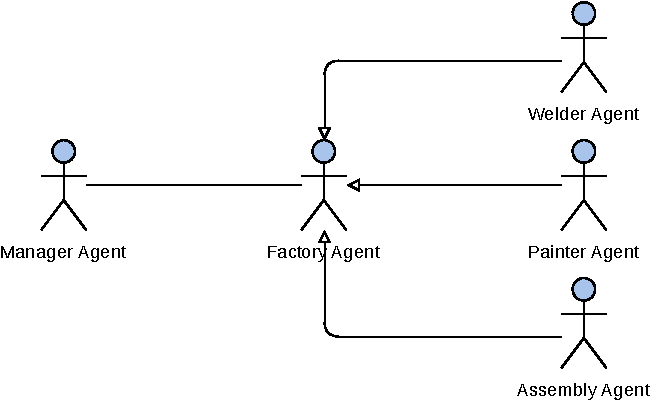
\includegraphics[width=\columnwidth]{figures/SAG-Agents.pdf}
    \caption{Dekompozycja systemu na agenty}
    \label{fig:agents}
\end{figure}

Agent \texttt{Manager Agent} zajmuje się zarządzaniem pracą w~fabryce. Do jego zadań należy:
\begin{itemize}
    \item zlecanie zadań,
    \item odbiór i~prezentacja wyników,
    \item monitorowanie działania pozostałych agentów.
\end{itemize}
W~systemie planowania pracy może znajdować się tylko jeden agent tego typu. Zarządca jest elementem krytycznym systemu, jego uszkodzenie powoduje błąd całego systemu.

Agent \texttt{Factory Agent} reprezentuje pojedynczą komórkę roboczą fabryki. To właśnie one realizują postawione zadanie planowania. Zadaniem agentów tego typu jest:
\begin{itemize}
    \item (pareto) optymalizacja lokalna sekwencji,
    \item negocjowanie z~innymi agentami tego typu,
    \item zgłaszanie problemów z~komunikacją do zarządcy.
\end{itemize}

W~celu prezentacji działania algorytmu zdecydowaliśmy się na stworzenie trzech oddzielnych komórek fabryki, reprezentowanych przez:
\begin{itemize}
    \item agenta spawalni \texttt{Welder Agent},
    \item agenta lakierni \texttt{Painter Agent},
    \item agenta stacji montażowej \texttt{Assembly Agent}.
\end{itemize}

\subsection{Dekompozycja agentów na zachowania}
Każdy agent składa się z~kilku zachowań działających współbieżnie. Zachowanie jest zadaniem, które agent może realizować w~powtarzalny sposób. Biblioteka \texttt{SPADE}~\cite{spade} udostępnia podstawowe typy zachowań:
\begin{itemize}
    \item \texttt{One-Shot} - jednorazowe zachowanie,
    \item \texttt{Cyclic} - cyklicznie uruchamiane zachowanie,
    \item \texttt{Timeout} - jednorazowe zachowanie, uruchamiane przez agenta w~wyszczególnionej chwili czasowej,
    \item \texttt{FSM} - umożliwia definiowanie zachowania przy użyciu skończonego automatu stanów.
\end{itemize}

Z~każdym zachowaniem, skojarzony jest szablon wiadomości. W~momencie przyjścia wiadomości, dla każdego zachowania, agent sprawdza czy wiadomość jest zgodna z~szablonem. Jeżeli wiadomość i~szablon, są ze sobą zgodne, to agent umieszcza wiadomość w~skrzynce odbiorczej danego zachowania, z~którego może ona zostać pobrana. 

\subsubsection{Agent nadzorujący}
Agent zarządczy \texttt{Manager Agent} składa się z~trzech zachowań, w~ramach których tworzone i~zarządzane są pozostałe agenty. Dekompozycja na poszczególne zachowania został przedstawiony na rysunku~\ref{fig:manager-behaviours}.

\begin{figure}[h]
    \centering
    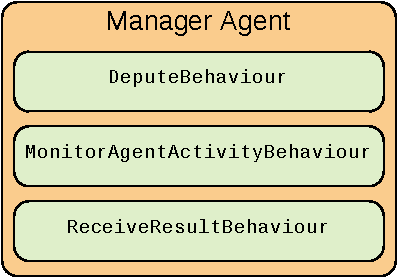
\includegraphics[width=0.8\columnwidth]{figures/SAG-Manager-Behaviours.pdf}
    \caption{Podział agenta \texttt{Manager Agent} na zachowania}
    \label{fig:manager-behaviours}
\end{figure}

Pierwszym zachowaniem jest \texttt{Depute}, którego rolą jest jednorazowe stworzenie wszystkich agentów oraz wysłanie im zadania, przedstawionego jako lista wszystkich końcowych produktów, wraz z~ich zadaną licznością.

Kolejnym zachowaniem jest \texttt{MonitorAgentActivity}. Rolą tego zachowania jest monitorowanie stanu stołu negocjacyjnego. Jeżeli agent reprezentujący daną komórkę fabryki wyczerpał swoje możliwości, zgłasza ten fakt do zarządcy, wykorzystując właśnie to zachowanie. Obecność tego zachowania pozwala na uniknięcie wyścigów krytycznych, czyli sytuacji podczas której wszyscy agenci równocześnie rezygnują z~dalszych negocjacji i~żaden z~nich nie wysyła informacji o~ostatecznym rozwiązaniu.

Ostatnim elementem agenta nadzorującego jest zachowanie \texttt{ReceiveResult}, które oczekuje na wiadomość z~ostatecznie ustaloną sekwencją działania. W~momencie otrzymania wyniku, agent wstrzymuje działanie wszystkich agentów w~systemie, prezentuje wynik i~zamyka program. 

\subsubsection{Agent komórki fabryki}
Agent typu \texttt{Factory Agent} składa się z~czterech, oddzielnych zachowań, które realizują różne funkcje w~systemie. Podział na zachowania został przedstawiony na rysunku~\ref{fig:factory-behaviours}.

\begin{figure}[h]
    \centering
    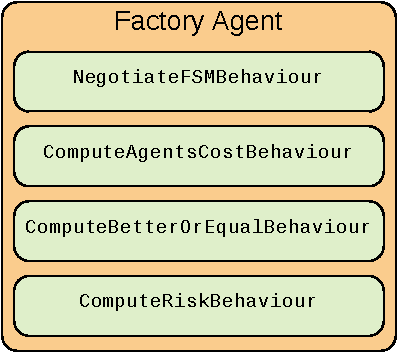
\includegraphics[width=0.8\columnwidth]{figures/SAG-Factory-Behaviours.pdf}
    \caption{Podział agenta \texttt{Factory Agent} na zachowania}
    \label{fig:factory-behaviours}
\end{figure}

Najważniejszym zachowaniem w~systemie jest zachowanie \texttt{NegotiateFSM}, które realizuje algorytm negocjacji pomiędzy agentami. Same negocjacje zostały zaimplementowane jako skończona maszyna stanów, która została przedstawiona na rysunku~\ref{fig:factory-fsm}.

\begin{figure}[h]
    \centering
    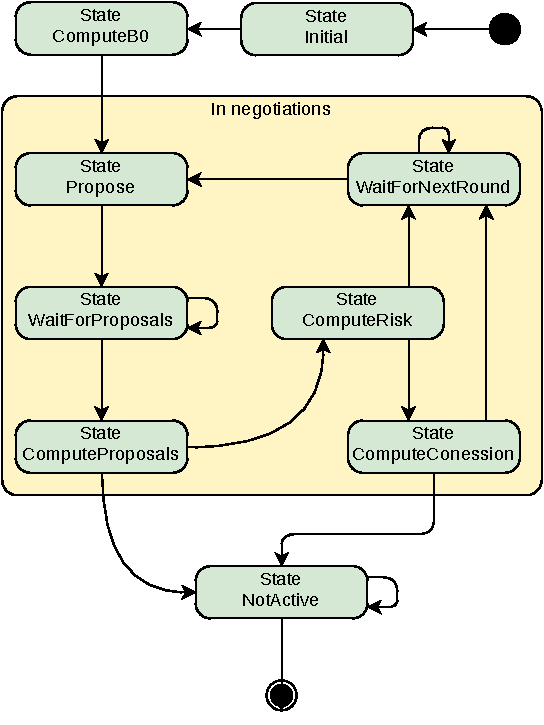
\includegraphics[width=\columnwidth]{figures/SAG-FactoryFSM.pdf}
    \caption{Maszyna stanów na której bazuje zachowanie \texttt{FSMBehaviour}}
    \label{fig:factory-fsm}
\end{figure}

Pozostałe zachowania są konieczne aby dany agent był w~stanie zbudować bazę wiedzy na temat możliwości pozostałych agentów.

Zachowanie \texttt{ComputeAgentsCost} pozwala na uzyskanie informacji, jak bardzo dobra dla danego agenta jest podana sekwencja.
Agenci odpytują się nawzajem, tak aby móc zaproponować rozwiązanie dobre dla wszystkich agentów w~systemie. 

Kolejnym zachowanie jest \texttt{ComputeBetterOrEqual}, które  umożliwia agentom uzyskać informację na temat zbioru znanych przez agenta rozwiązań problemu, których koszt jest mniejszy lub równy od podanego. Innymi słowami, pozwala na otrzymanie wszystkich rozwiązań które są lepsze lub co najmniej tak dobre jak podane.

Ostatnim zachowaniem jest \texttt{ComputeRisk} jest wykorzystywane przy szukaniu kompromisu. Agenci odpytują się nawzajem, przy użyciu tego zachowania, aby znaleźć agenta który ma \textit{najmniej} do stracenia, czyli tego którego wzrost kosztu przy odpuszczeniu będzie najmniejszy.